%=======================+=========================
%================  Performance  ================
%=================================================

\section[Detector performance]{Detector performance \label{sec:performance}}

The performance of the GlueX detector to reconstruct charged and neutral particles and assemble them into fully reconstructed events has been studied in data and simulation using several photoproduction reactions.  The results of these studies are summarized in this section.

%\subsection{Charged particles \label{sec:perfcharged}}

%\subsubsection{Efficiency \label{sec:perfchargedeff}}

%The reconstruction efficiency for different hadron species has been studied using the method described in Sec.~\ref{sec:trackeff}.   Charged pion reconstruction efficiency was studied with a sample of $\gamma p \to p \omega$, $\omega \to \pi^+\pi^-\pi^0$ events.  Charged kaon reconstruction efficiency was studied with samples of $\gamma p \to \phi p$, $\phi \to K^+K^-$ and $\gamma p \to \Lambda(1520) K^+$, $\Lambda(1520) \to p K^-$ events.  Proton reconstruction efficiency was studied with a sample of $\gamma p \to K^+ \Sigma^0$, $\Sigma^0 \to \gamma \Lambda^0$, $\Lambda^0 \to p \pi^-$ events.  
%The results are illustrated in Fig.~X. The efficiencies determined by data and simulation generally agree to within a few percent.

\subsection{Charged particle reconstruction efficiency  \label{sec:trackeff}}

We estimated the track reconstruction efficiency by analyzing $\gamma p \rightarrow p \omega$, $\omega\rightarrow\pi^+\pi^-\pi^0$ events where we used the proton, the $\pi^0$ and one of the charged pions to predict the three-momentum of the other charged pion. We used two methods to calculate this efficiency, $\varepsilon=N_{found}/(N_{found}+N_{missing})$.  Events for which no track is reconstructed in the predicted region of 
phase space contribute to $N_{missing}$, while events where the expected track was found to be reconstructed contribute to $N_{found}$.  For the first method, the $\omega$ yields for $N_{found}$ and $N_{missing}$ was estimated from the missing mass off the 
proton; for the second method, the invariant mass of the $\pi^+\pi^-\pi^0$ system was used to find $N_{found}$.  This analysis was performed individually in bins of track momentum, $\theta$, and $\phi$.
Examples of mass histograms for a particular bin in $\phi$ are shown in Fig.~\ref{fig:omega mass}.  The exercise was repeated for a sample of $\omega$ Monte Carlo events.   A comparison of the efficiency for pion reconstruction derived from the 
two methods for both Monte Carlo and experimental data is shown in Fig.~\ref{fig:tracking efficiency}.  The efficiencies for Monte Carlo and experimental data 
agree within 5\%.

While this reaction only allows the determination of track reconstruction efficiencies for $\theta < 30^\circ$, this covers the majority of charged particles produced in GlueX due to its fixed-target geometry.  Other reactions are being studied to determine the efficiency at larger angles.

\begin{figure}[tbp]
\begin{center}
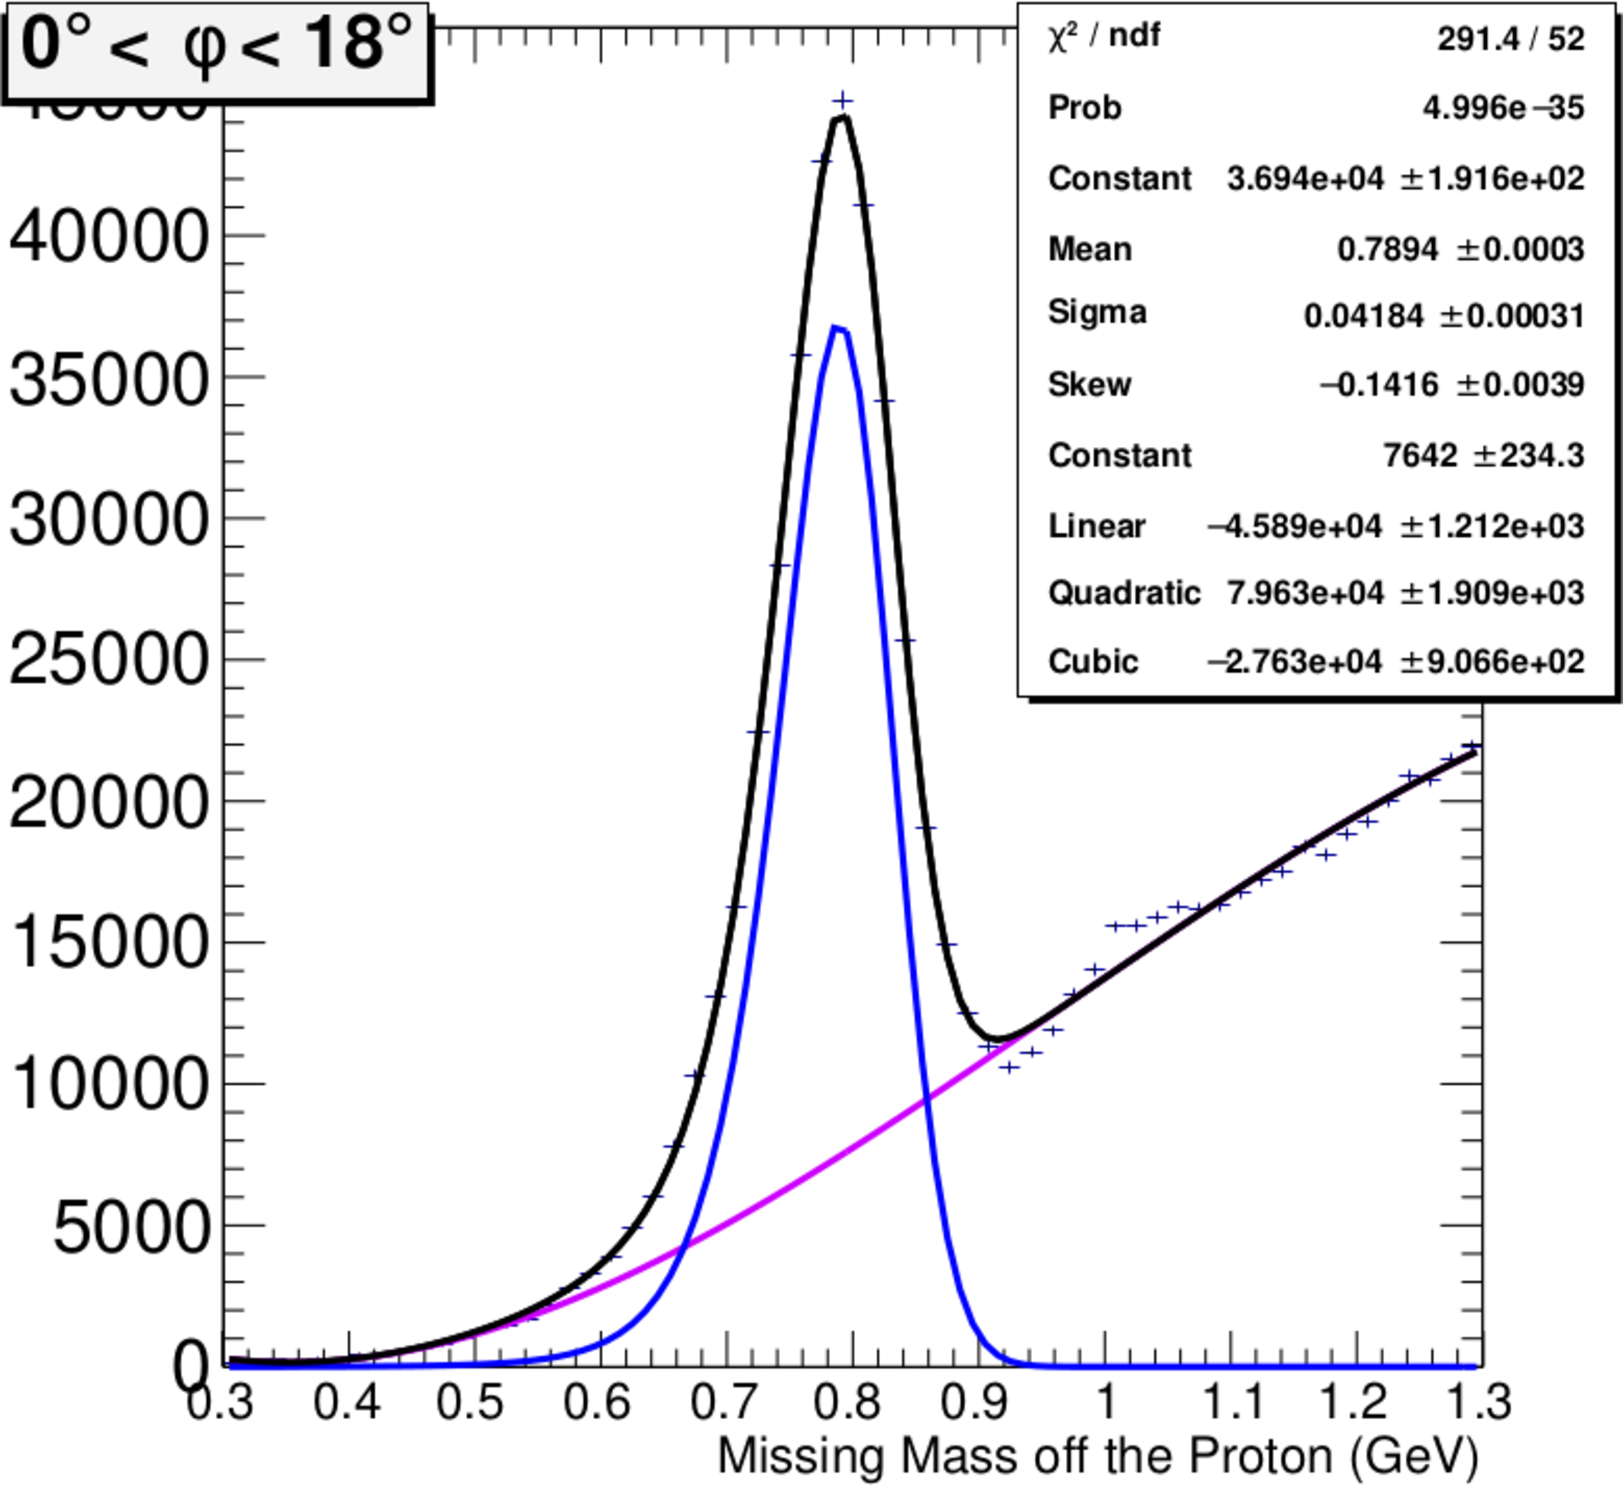
\includegraphics[width=0.45\textwidth]{figures/MissingOmegaFit.pdf}
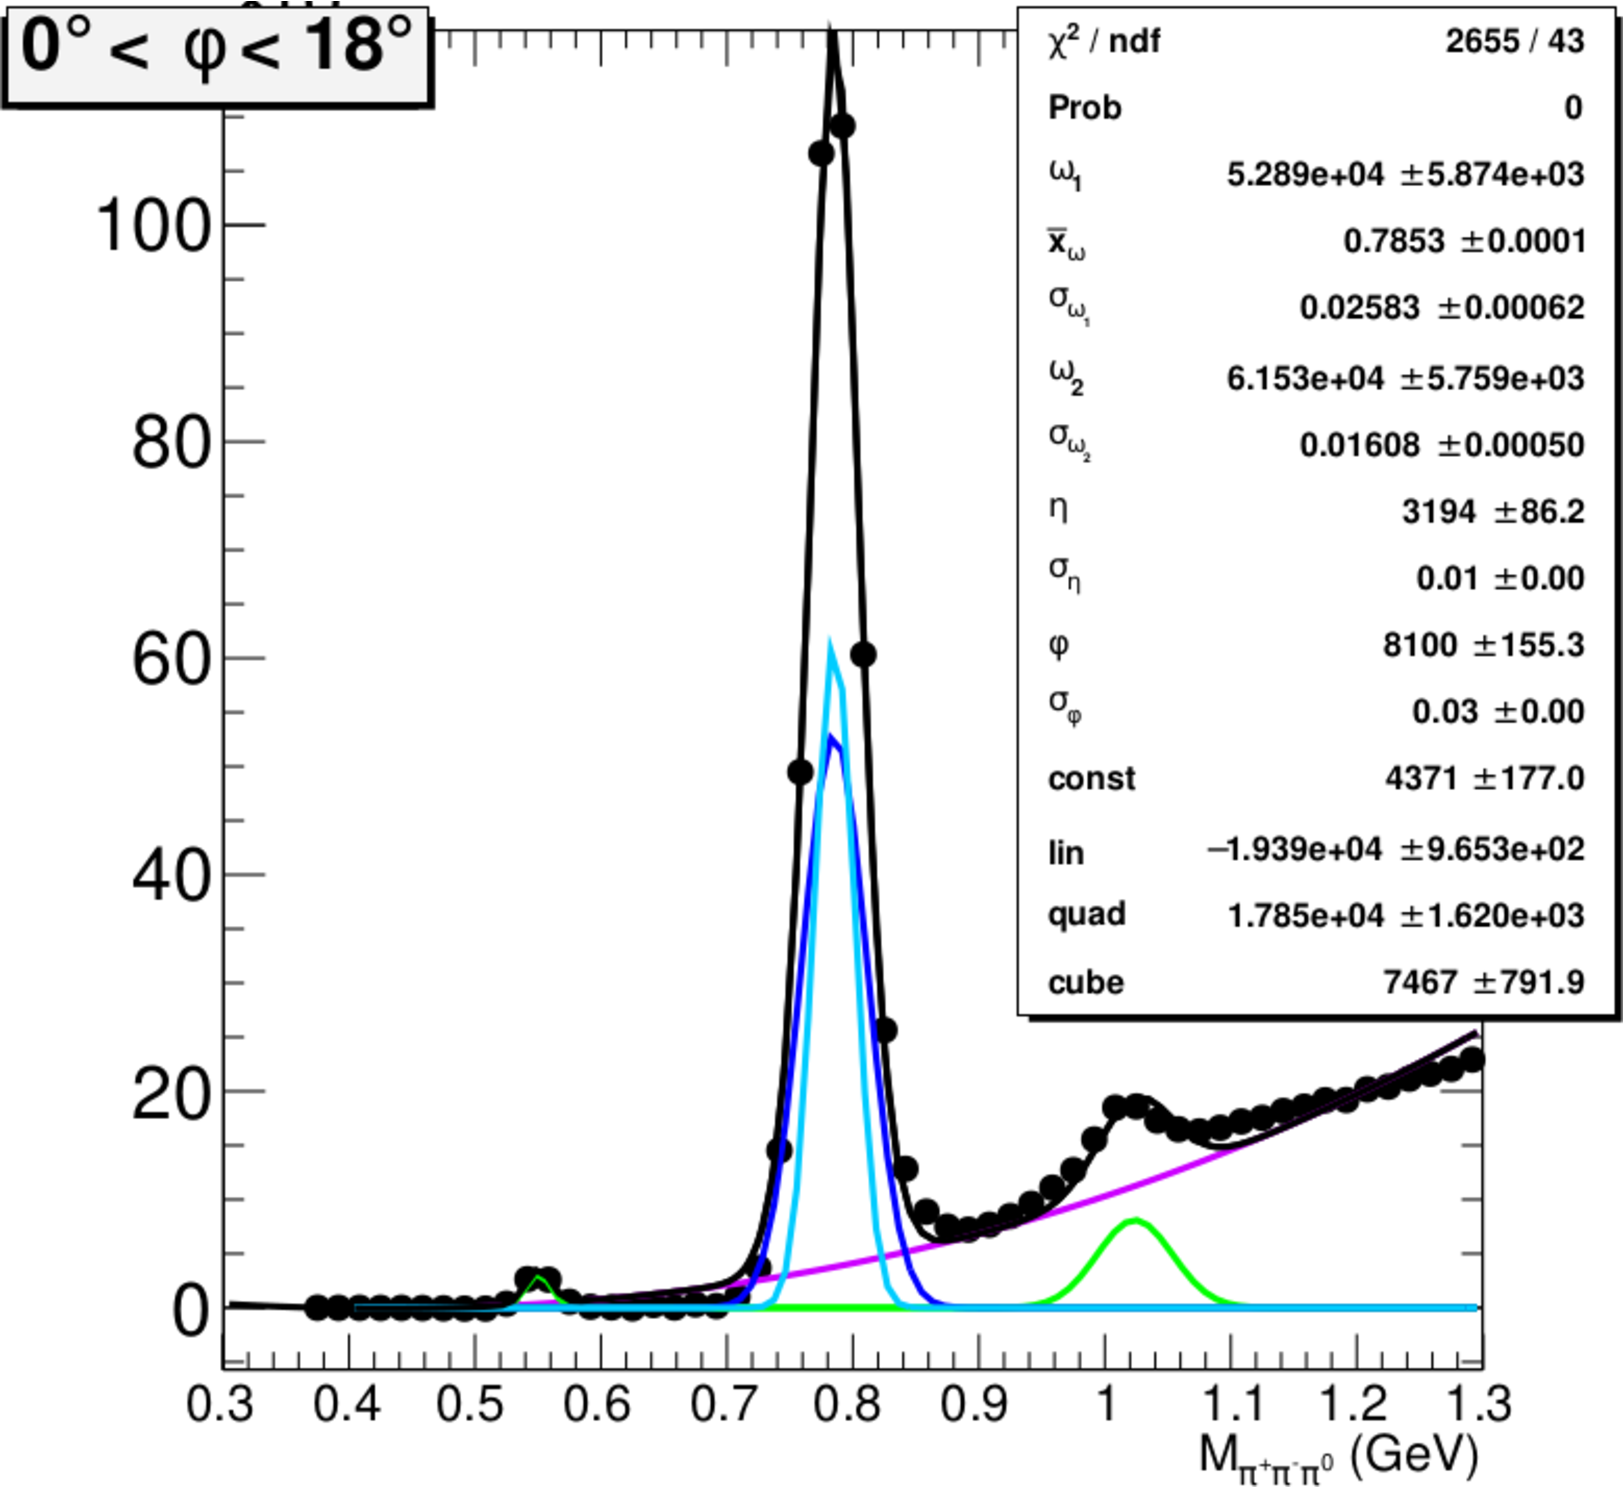
\includegraphics[width=0.45\textwidth]{figures/ThreePiFit.pdf}
\caption{\label{fig:omega mass}
Reconstructed mass distributions for the reaction $\gamma p \to p\pi^0\pi^{\pm}(\pi^\mp)$ for a bin in $\phi$.
  (Left) Distribution of the missing mass off the proton.
(Right) Invariant mass distribution for the $\pi^+\pi^-\pi^0$ system.  The black
curves show the results of fits to the distributions.
 (Color online)}
\end{center}
\end{figure}

\begin{figure}[tpb]
\begin{center}
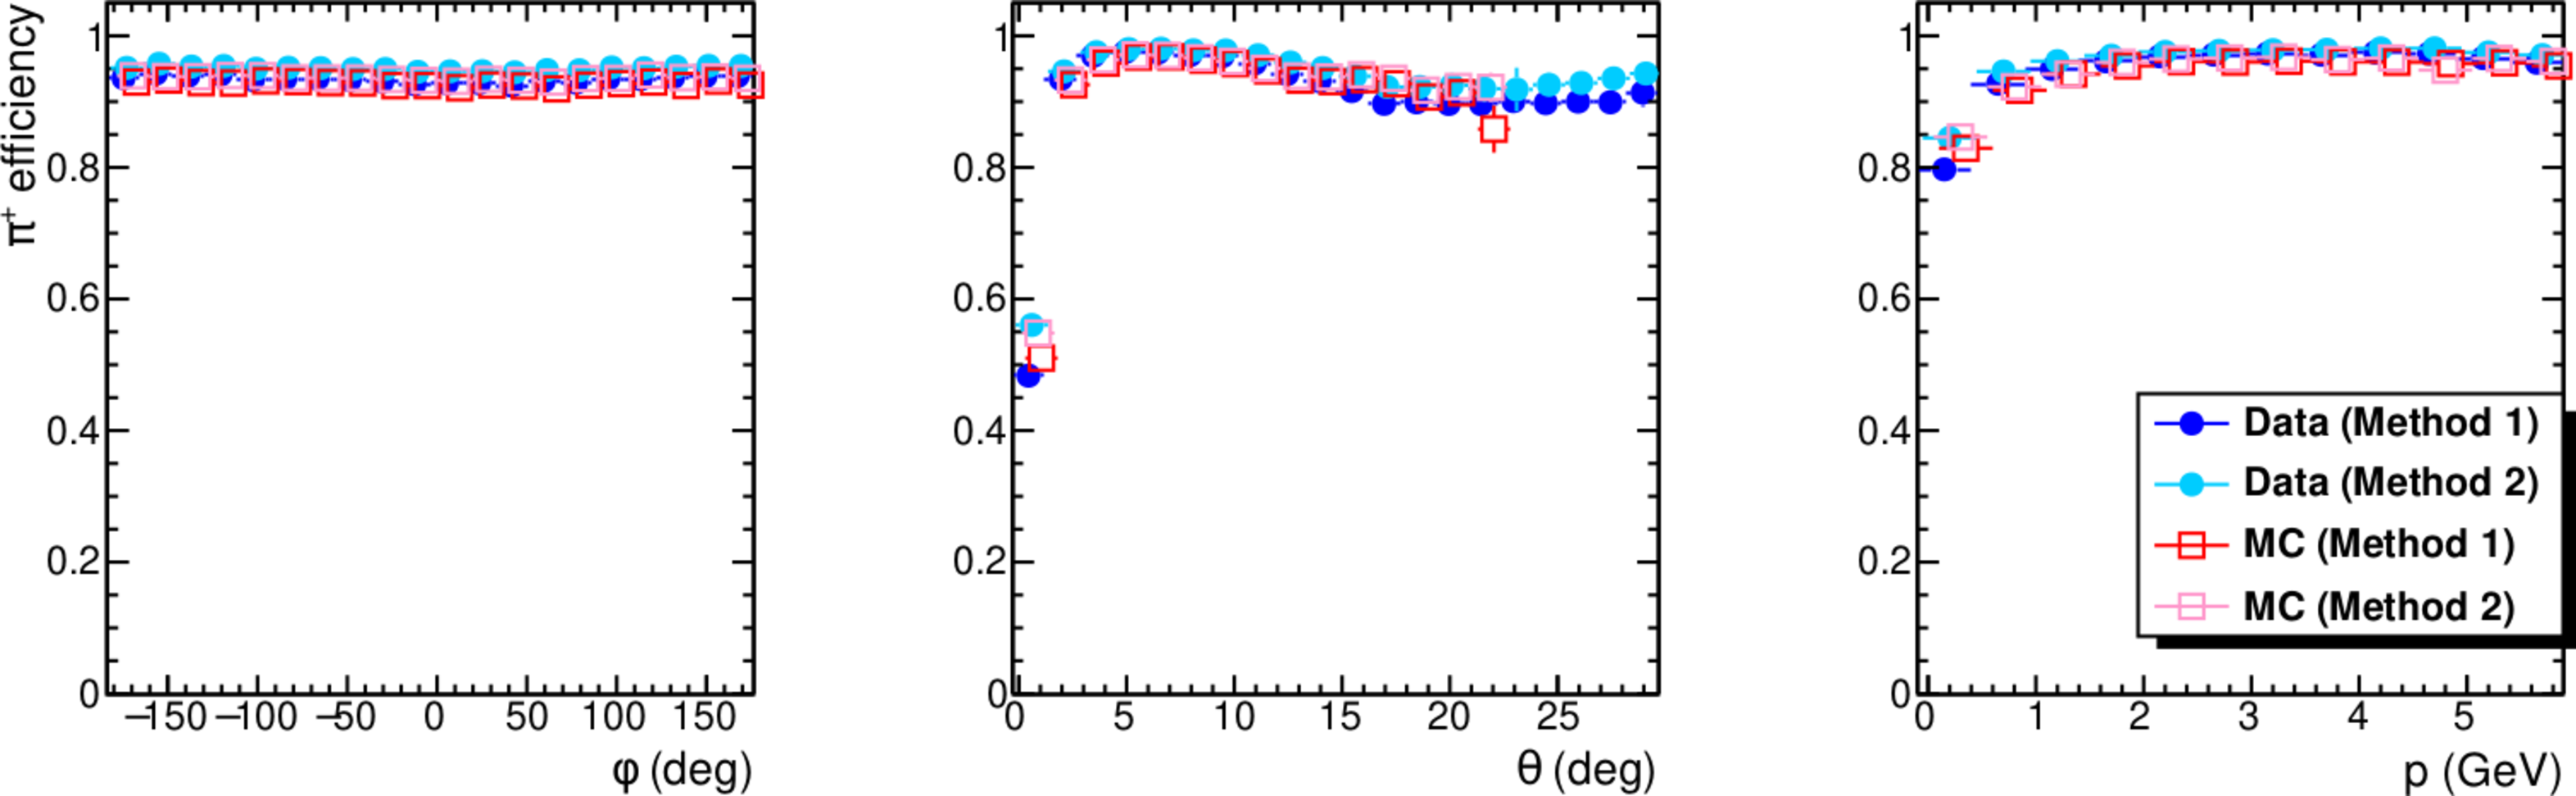
\includegraphics[width=\textwidth]{figures/PiPlusEfficiency.pdf}
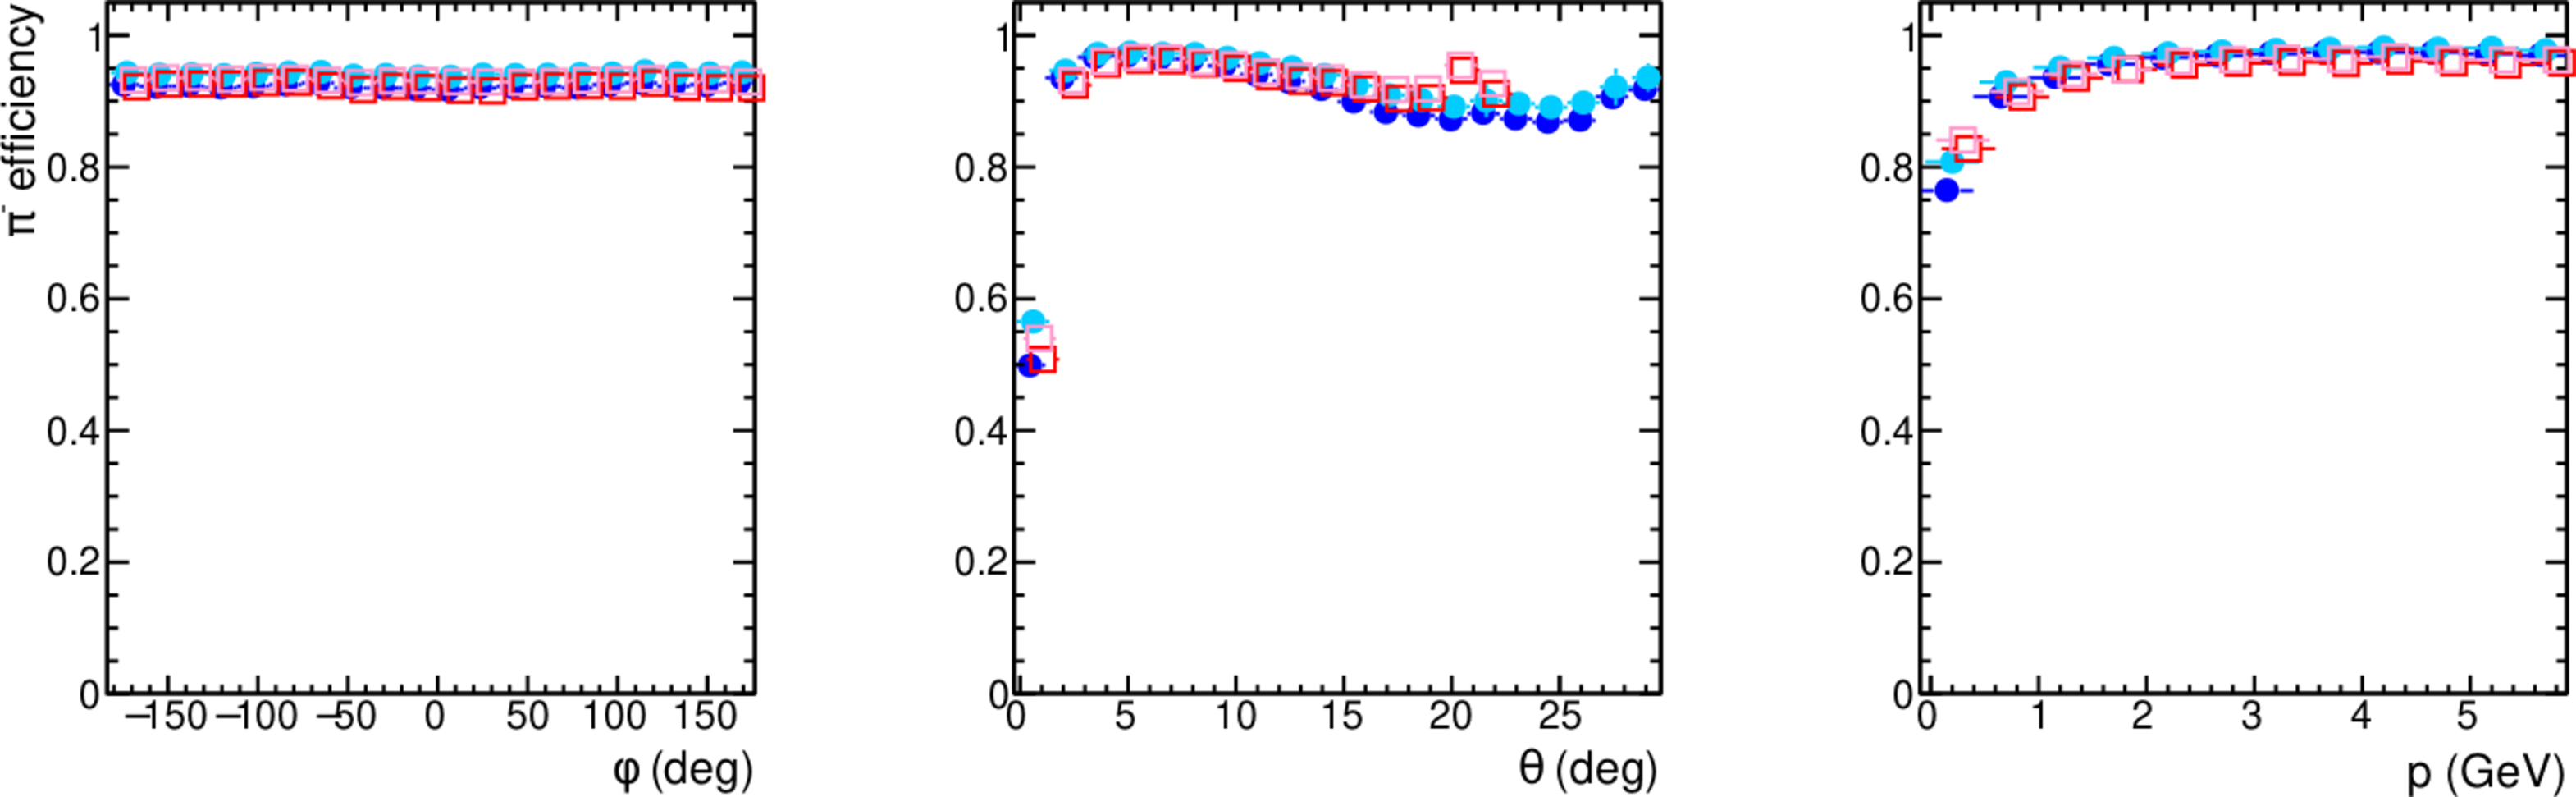
\includegraphics[width=\textwidth]{figures/PiMinusEfficiency.pdf}
\caption{\label{fig:tracking efficiency}
(Top row) Tracking efficiency for $\pi^+$ tracks. (Bottom row) Tracking efficiency for $\pi^-$ tracks.  (Color online)}
\end{center}
\end{figure}


\subsubsection{Invariant Mass Resolution \label{sec:perfchargedresol}}

The invariant mass resolution for resonances decaying into charged particles depends on the momenta and angles of the various decay products.  This resolution has been studied using several different channels:  $K_S\to\pi^+\pi^-$ from $\gamma p \to K_S K^+ \pi^- p$; $\eta \to \pi^+\pi^-\pi^0$ from $\gamma p \to \eta p$; $\Xi^- \to \pi^- \Lambda^0$, $\Lambda^0 \to p \pi^-$ from $\gamma p \to K^+ K^+ \Xi^-$; and $J/\psi \to e^+ e^-$ from $\gamma p \to J/\psi p$.  The results are illustrated in Figs.~\ref{fig:invmass1} and \ref{fig:invmass2}.    In each case, the invariant mass resolution is in the range $4-15$~MeV, after applying a kinematic fit to the full reaction.

\begin{figure}[tpb]
\begin{center}
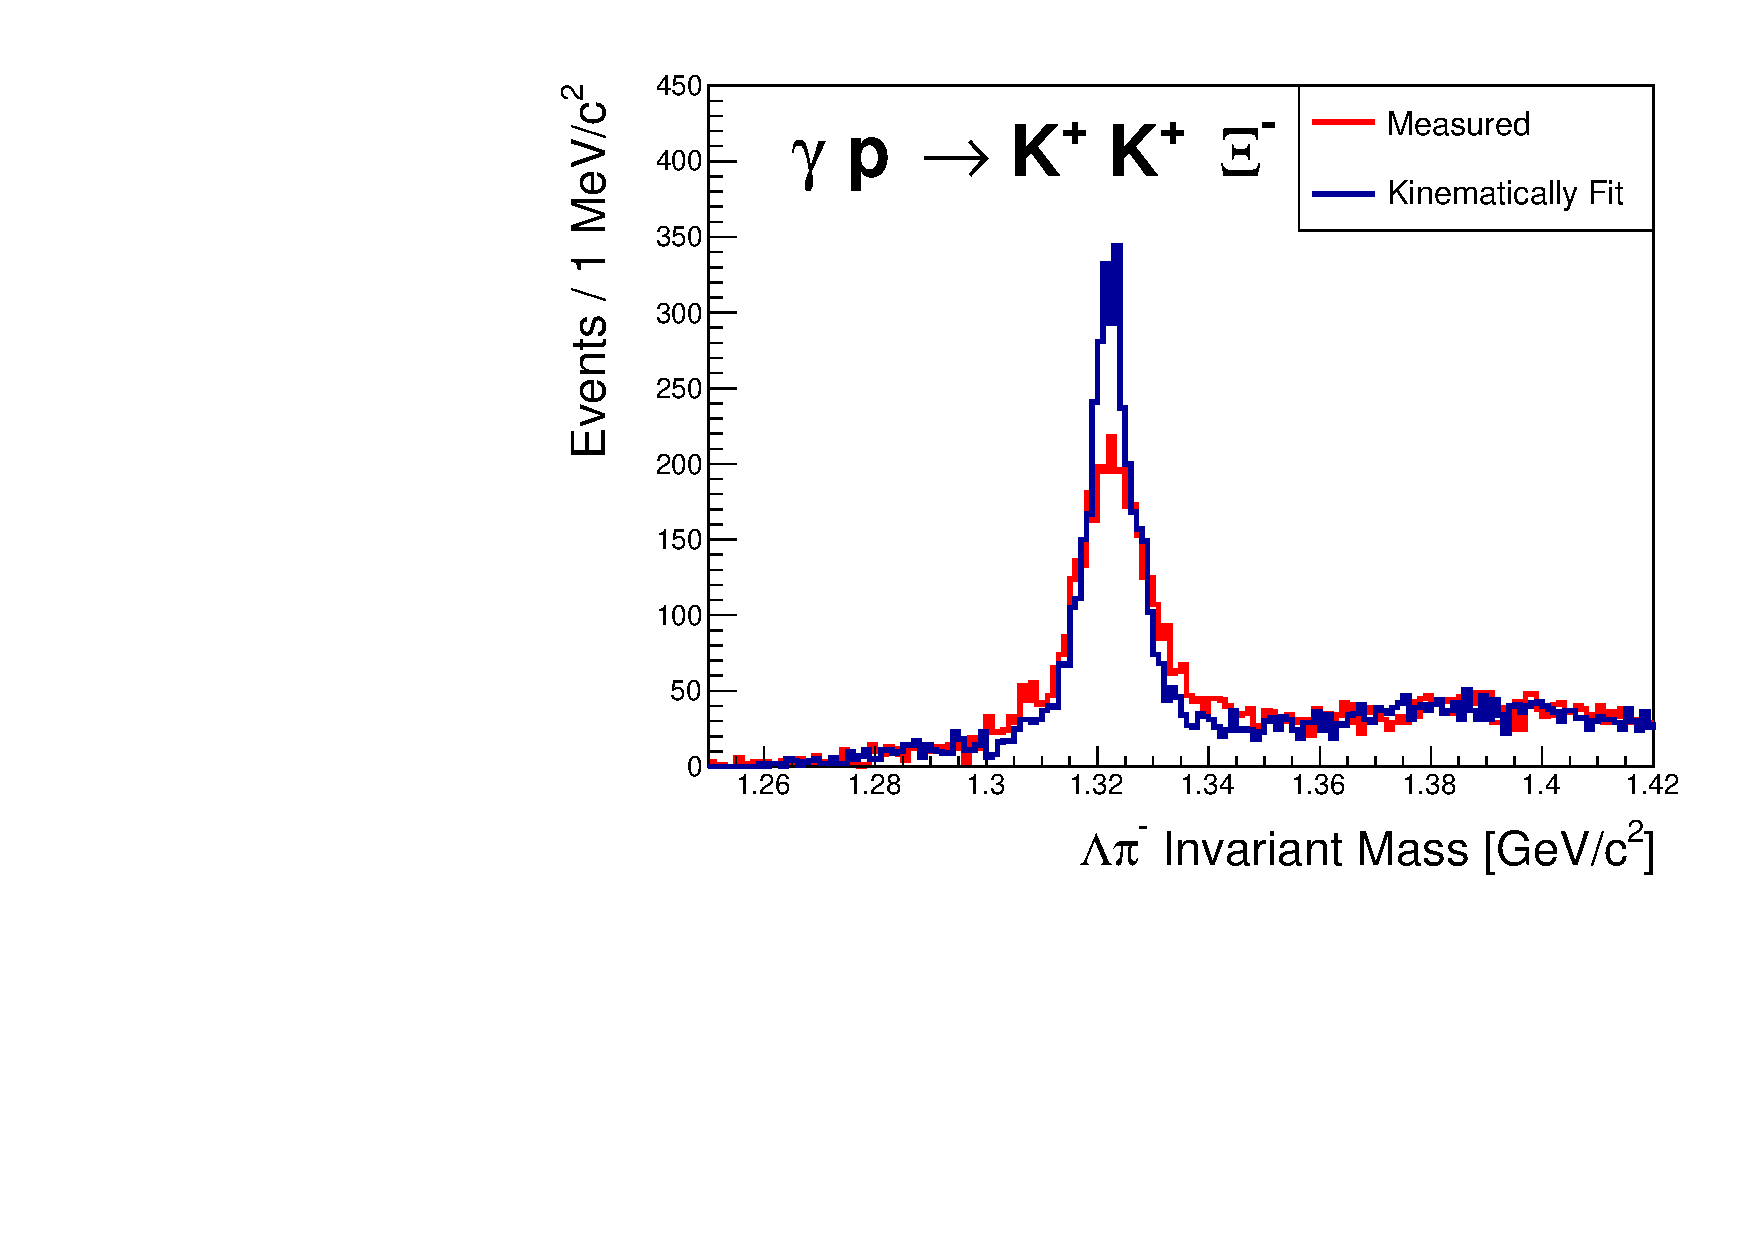
\includegraphics[width=0.42\textwidth]{figures/XimMass_2017-ver30.pdf}
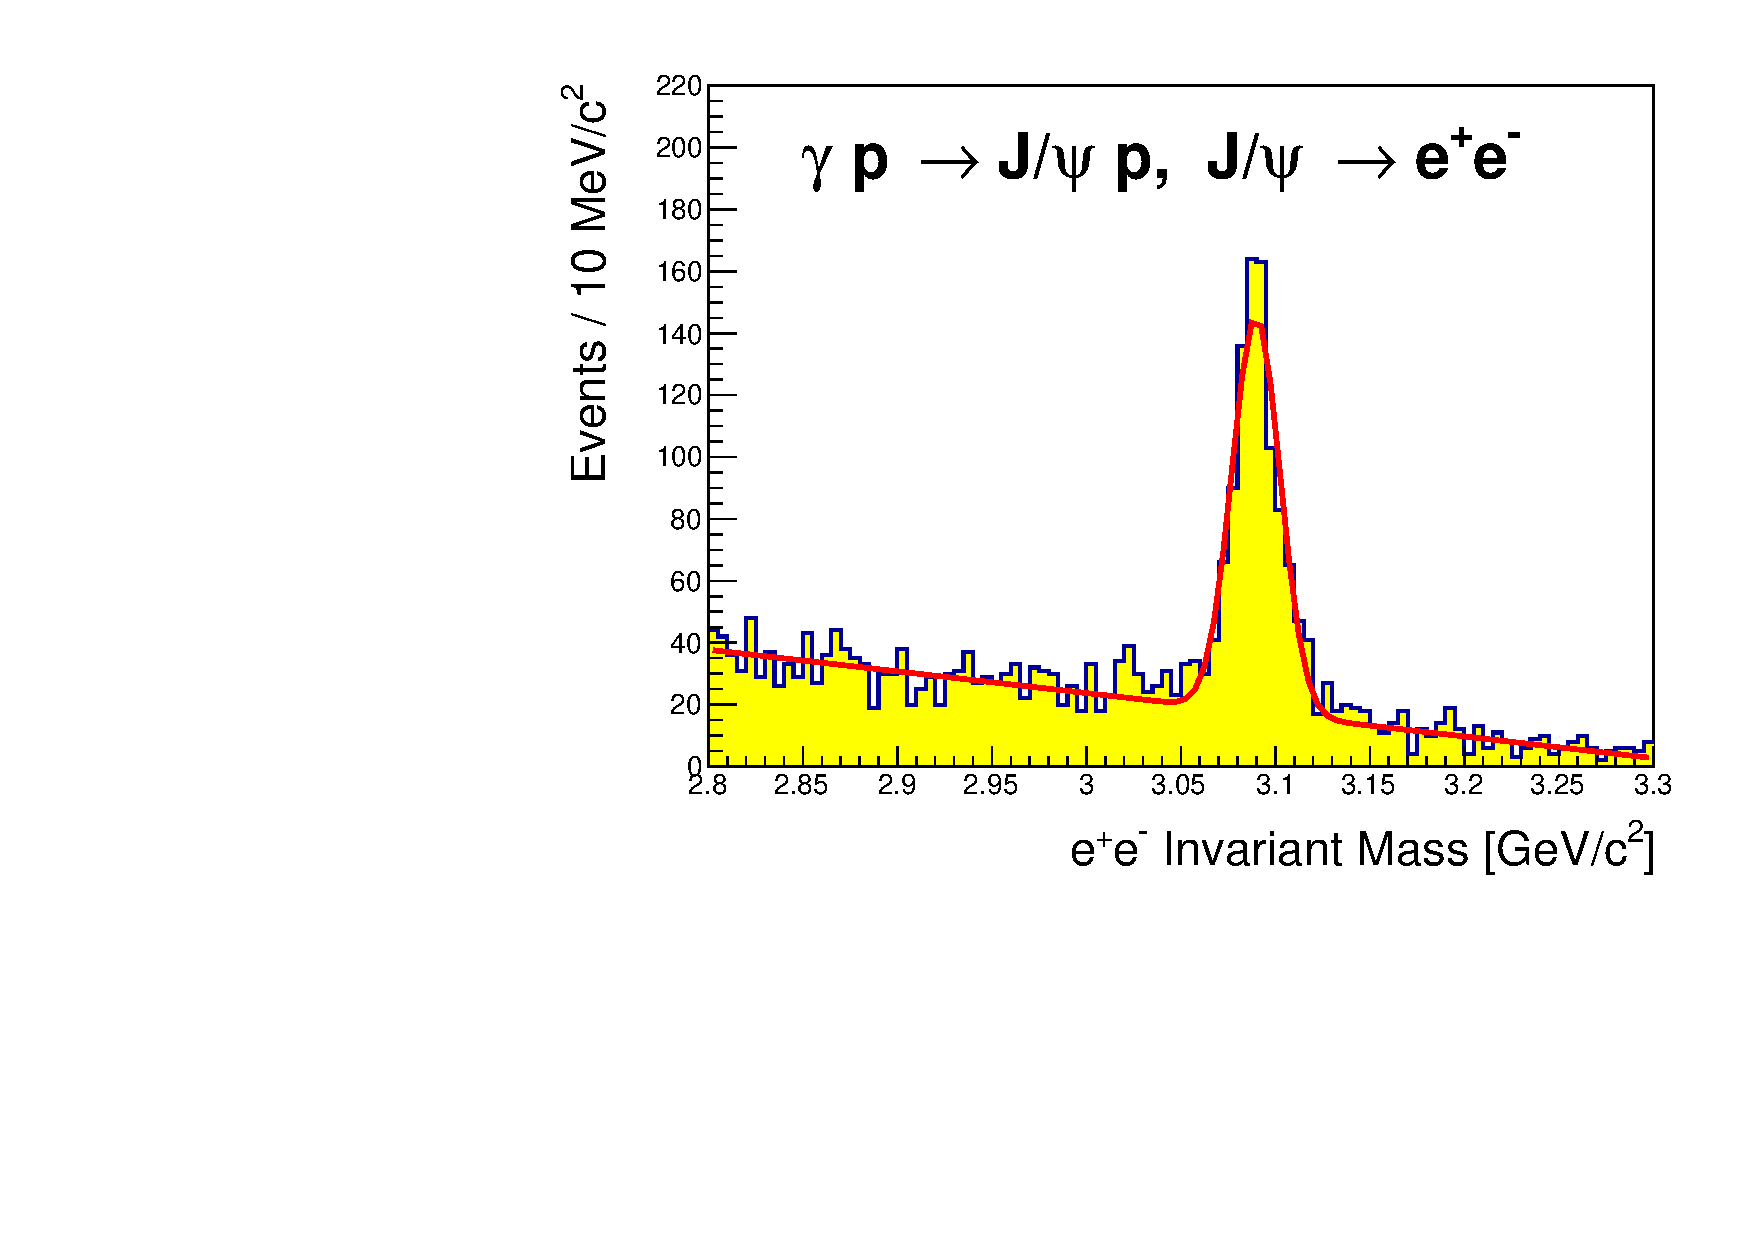
\includegraphics[width=0.42\textwidth]{figures/jpsi_mass.pdf}
\caption{\label{fig:invmass1}
(Left) $\Lambda^0\pi^-$ invariant mass distribution from $\gamma p \to K^+ K^+ \pi^- \pi^- p$ events, illustrating the peak due to $\Xi^- \to \pi^- \Lambda^0$, $\Lambda^0 \to p \pi^-$ events.  The $\Xi^-$ peak resolution is 7.3~MeV using just the reconstructed charged particle 4-vectors, and is 4.6~MeV after a kinematic fit imposing energy and momentum conservation and an additional constraint that the mass of the $p \pi^-$ pairs be that of the $\Lambda^0$ mass,   (Right) $e^+e^-$ invariant mass distribution from kinematically fit $\gamma p \to e^+e^- p$ events, illustrating the peak due to $J/\psi\to e^+e^-$ events.  The peak resolution is 13.7~MeV. (Color online)}
\end{center}
\end{figure}

\subsection{Neutral Particle Efficiency\label{sec:perfneutral}}

%\subsubsection{Resolution \label{sec:perfneutralresol}}

%The invariant mass resolution of the decay $\eta \to \gamma \gamma$ has been found to primarily depend on the energy resolution of the calorimeters at GlueX.  Therefore, in Fig.~X we show the resolution for these reconstructed decays for three classes of events: where both photons from the  $\eta \to \gamma \gamma$ are reconstructed in the BCAL, were both are reconstructed in the FCAL, and where one photon is reconstructed in the BCAL and one in the FCAL.

%\subsubsection{Efficiency \label{sec:perfneutraleff}}

Photon reconstruction efficiency has been studied using different methods for the FCAL and BCAL.  In the FCAL, absolute photon reconstruction efficiencies have been determined using the ``tag-and-probe'' method with a sample of photons from the reaction $\gamma p \to \omega p$, $\omega \to \pi^+\pi^-\pi^0$, $\pi^0 \to \gamma (\gamma)$, where one final photon is allowed but not required to be reconstructed.  The yields with and without the reconstructed photon are determined using two methods.  In the first method, the $\omega$ yield is determined from the missing mass spectrum, $M_X(\gamma p \rightarrow pX)$, selecting on whether only one or when both reconstructed photons are consistent with a final-state $\pi^0$. In the second method,  the count when both photons are found is determined from the $\omega$ yield from the fully reconstructed invariant mass $M(\pi^+\pi^-\gamma\gamma)$. If the photon is not reconstructed, the $\omega$ yield is determined by a fit to the distribution of the missing mass off of the proton.  Both methods yield consistent results, with a reconstruction efficiency generally above 90\%, and agree with the efficiencies determined from simulation better than 5\%.

\begin{figure}[tbp]
\begin{center}
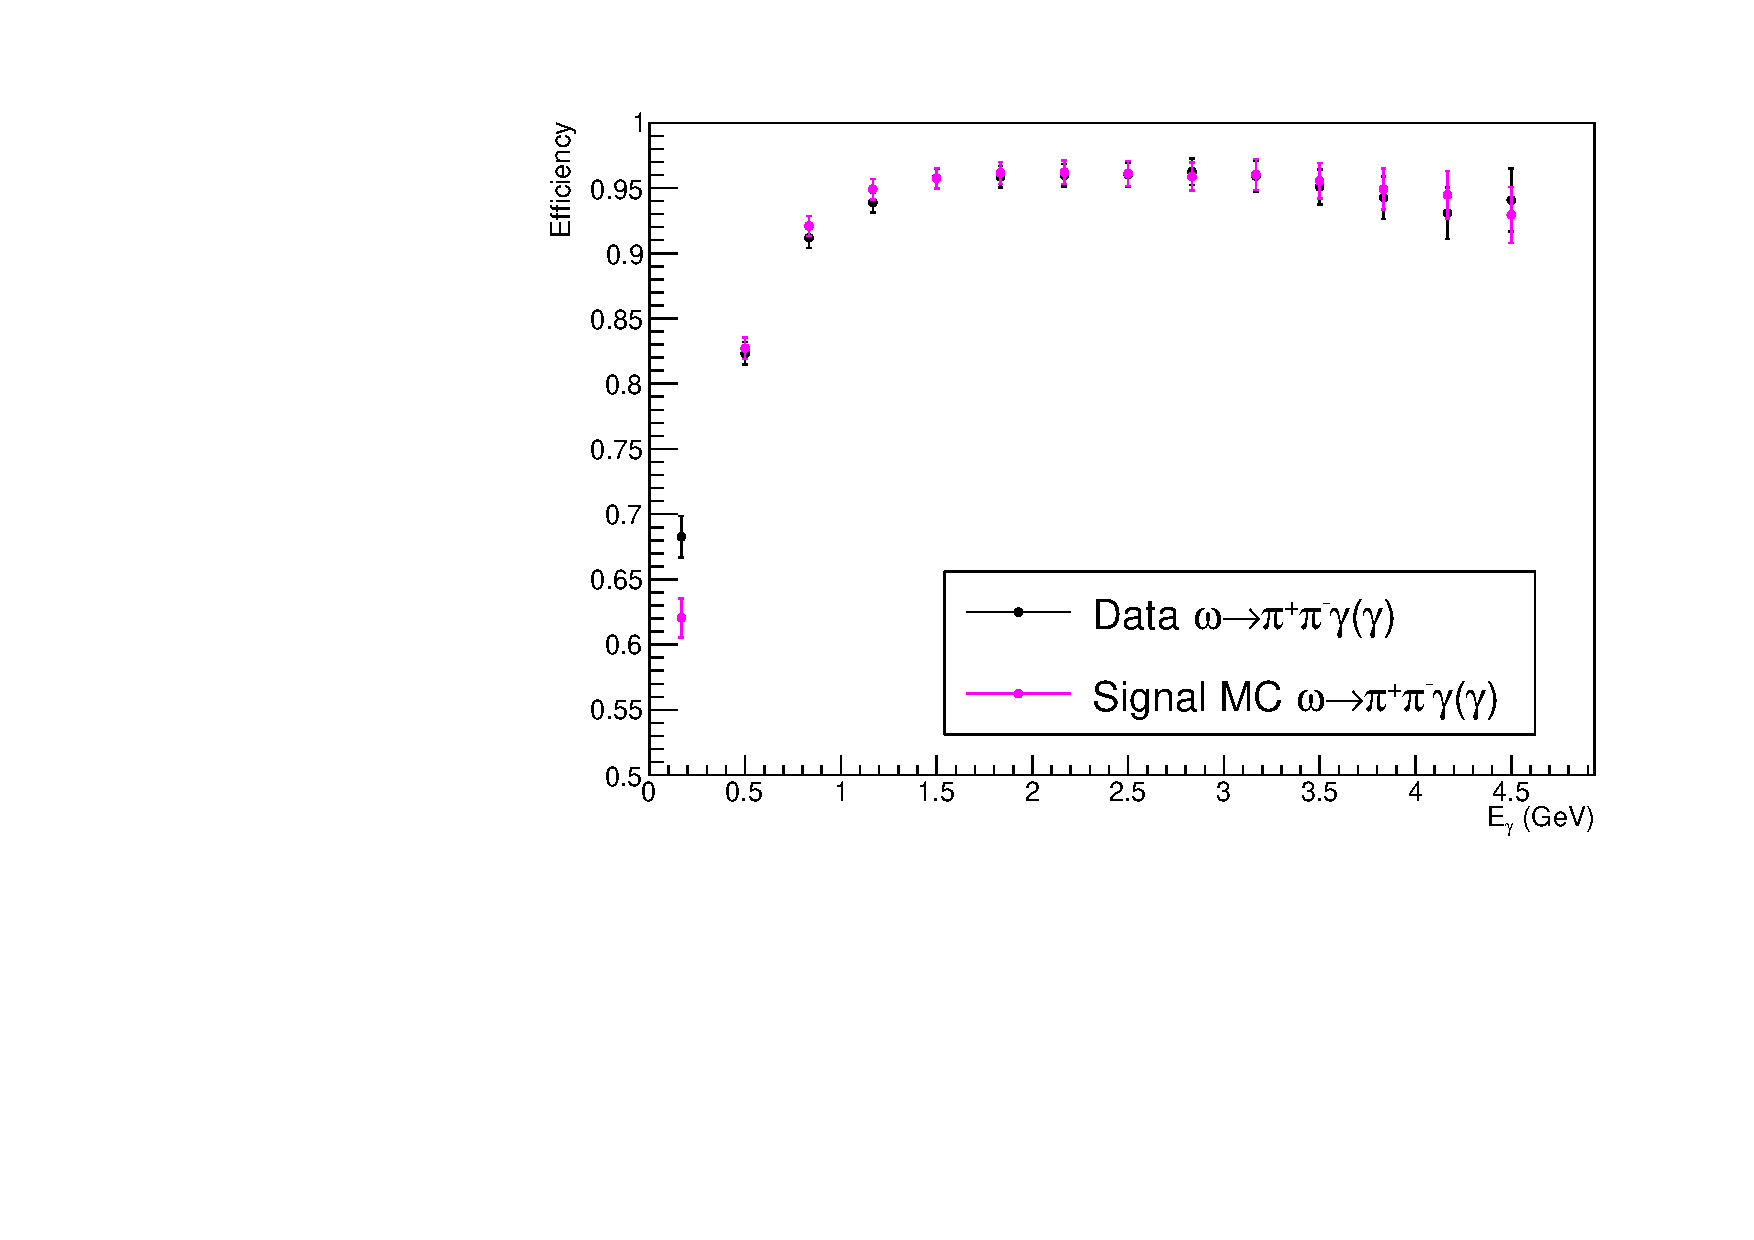
\includegraphics[width=0.45\textwidth]{figures/OmegaCompareE.pdf}
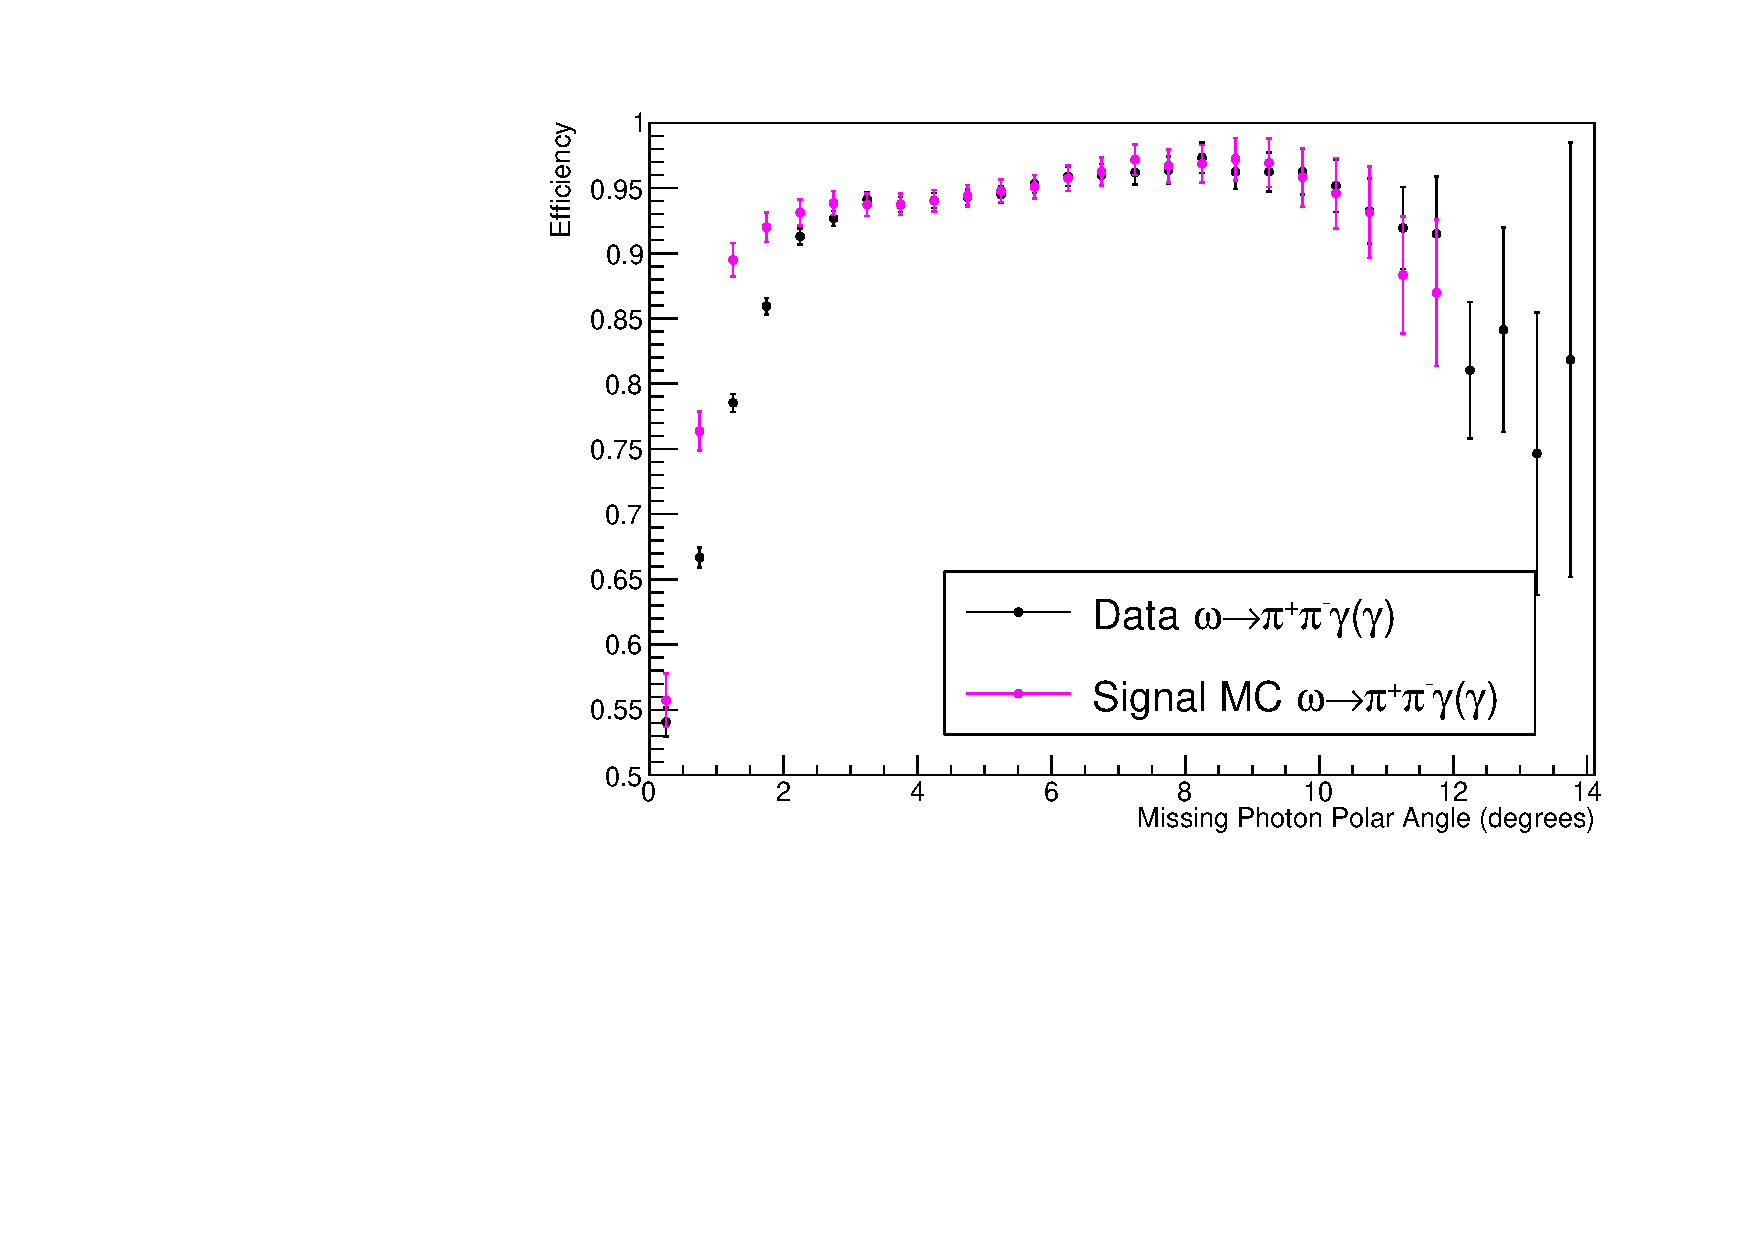
\includegraphics[width=0.45\textwidth]{figures/OmegaCompareTheta.pdf}
\caption{\label{fig:fcalphotoneff}
Photon reconstruction efficiency in FCAL determined from $\gamma p \to \omega p$, $\omega \to \pi^+\pi^-\pi^0$, $\pi^0 \to \gamma (\gamma)$ as a function of (left) photon energy and (right) photon polar angle.  Good agreement between data and simulation is observed in the fiducial region $\theta = 2^\circ - 10.6^\circ$.
 (Color online)}
\end{center}
\end{figure}

A relative photon efficiency determination has been performed using $\pi^0\to\gamma\gamma$ decays which spans the full angular range detected in GlueX.  We look at a sample of fully reconstructed $\gamma p \to  \pi^+\pi^-\pi^0 p$ events, and use the fact that the $\pi^0\to\gamma\gamma$ decay is isotropic in the center of mass frame.  Therefore, any anisotropy reflects an inefficiency in the detector. Results from this analysis are illustrated in Fig.~\ref{fig:bcalpi0photoneff}. Generally, this relative efficiency is above 90\%, and agrees with that determined from simulation better than 5\%.  

The models for the simulated response of both calorimeters are in the process of being updated, and the final agreement between photon efficiency determined in data and simulation is expected to improve.

\begin{figure}[tbp]
\begin{center}
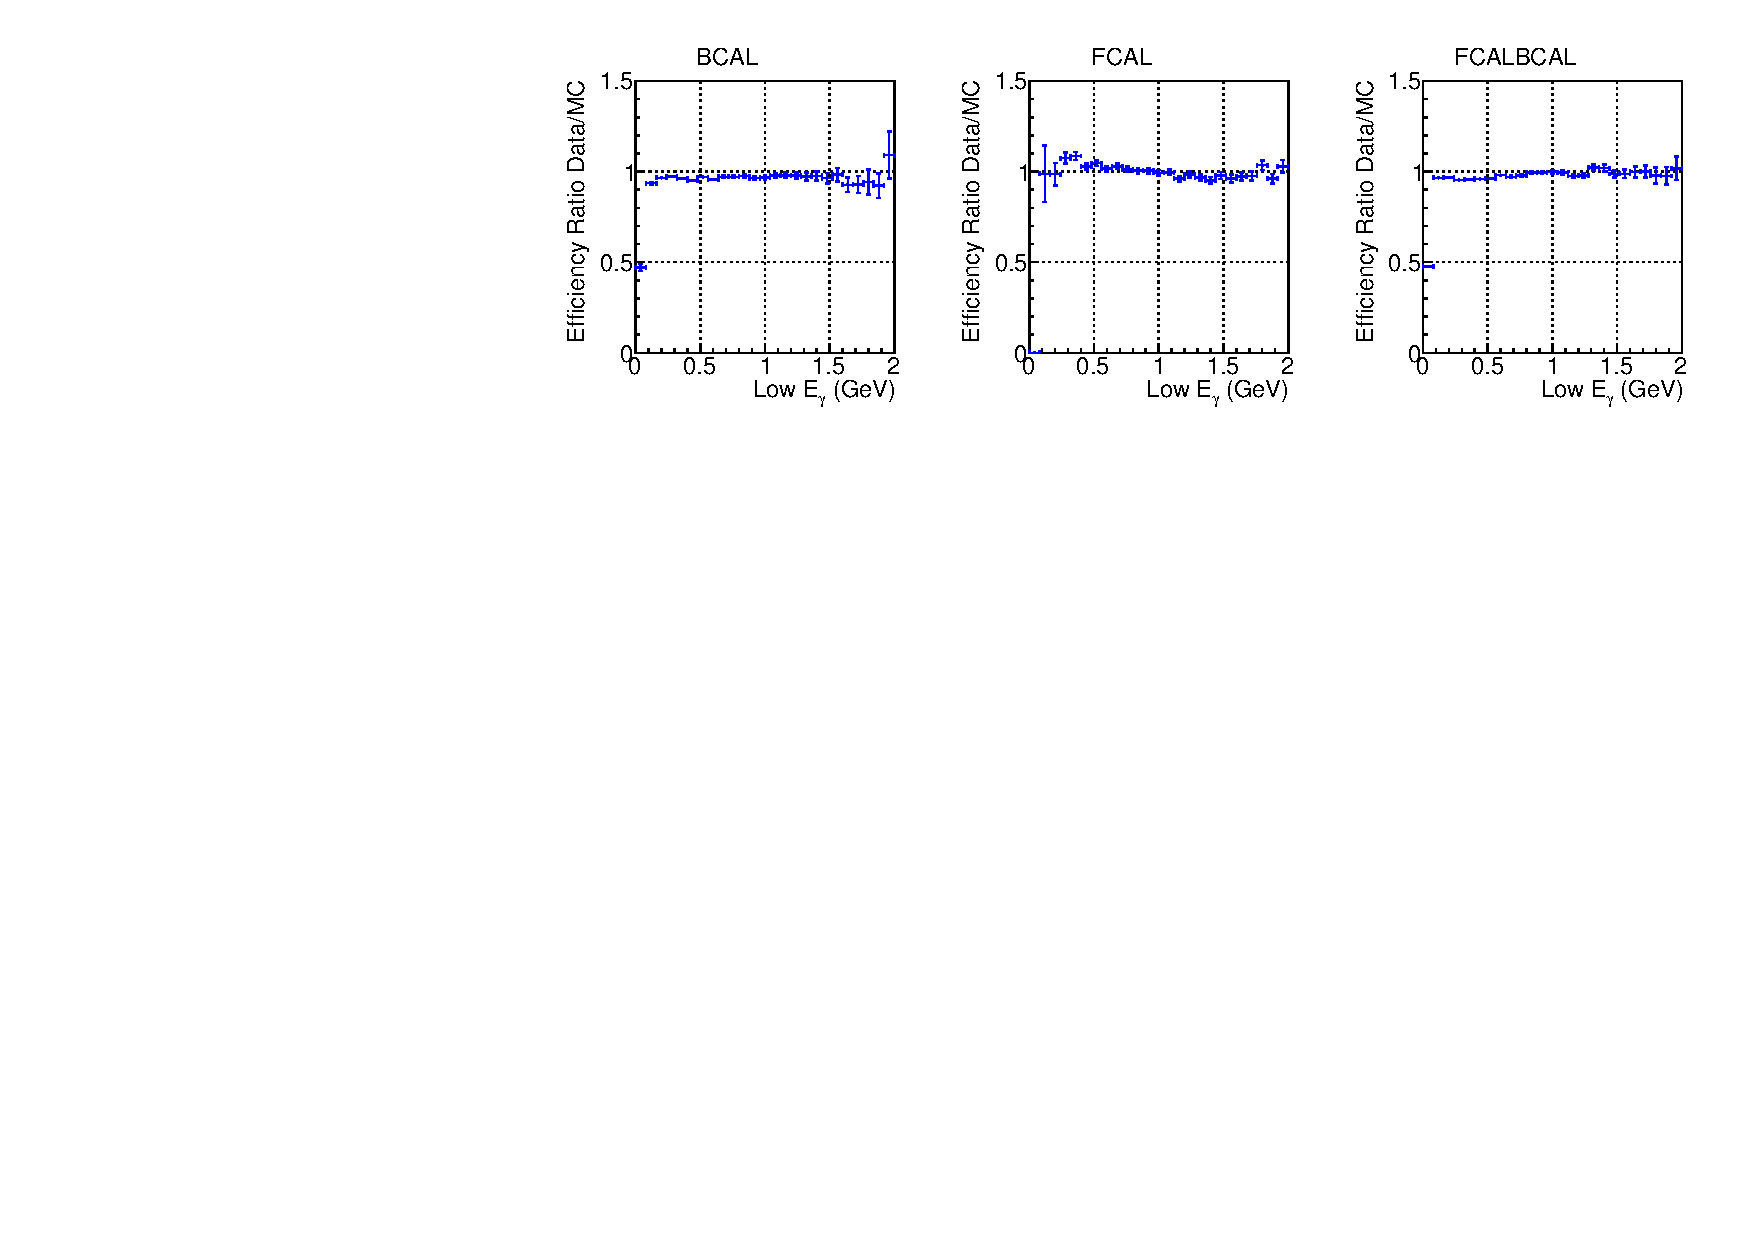
\includegraphics[width=\textwidth]{figures/plot_CostheEff_NIM_jun19.pdf}
\caption{\label{fig:bcalpi0photoneff}
Ratios of relative photon reconstruction efficiency between data and simulation determined from $\pi^0\to\gamma \gamma$ decays in $\gamma p \to  \pi^+\pi^-\pi^0 p$ events.  The efficiency ratios are shown for the cases where (left) both photons were measured in the BCAL, (middle) both photons were measured in the FCAL, and (right) one photon was measured in the BCAL and the other in the FCAL.
 (Color online)}
\end{center}
\end{figure}


Detailed studies of detector performance determined the standard fiducial region for most analyses to be $\theta = 2^\circ - 10.6^\circ$ and $\theta > 11.3^\circ$.  These requirements avoid the region dominated by beam-related backgrounds at small $\theta$ and the transition region between the BCAL and FCAL, where shower reconstruction is difficult.

\subsection{Kinematic fitting \label{sec:perffitting}}

Kinematic fitting is a powerful tool to improve the resolution of measured particles and to distinguish between different reactions.  In GlueX, this method leverages the fact that the initial state is very well known, with the target proton essentially at rest, and the incident photon energy is measured with very high precision ($<0.1\%$).  The most common kinematic fits that are performed are those that impose energy-momentum conservation between the initial and final state particles.  Additional optional constraints in these fits are for the four-momenta of the daughters of an intermediate particle to add up to a fixed invariant mass, and for all the particles to come from a common vertex (or multiple vertices, in the case of reactions containing long-lived, decaying particles).

To illustrate the performance of the kinematic fit, we first note that the improvement in the invariant mass resolution was seen to be $\approx20\%?$ for common reactions studied at GlueX. 
%we show the improvement in the invariant mass resolution in the reaction $\gamma p \to \eta p$, $\eta \to \pi^+\pi^-\pi^0$ in Fig.~X, and the pull distributions from the fit are illustrated in Fig.~X2.

\begin{figure}[tbp]
\begin{center}
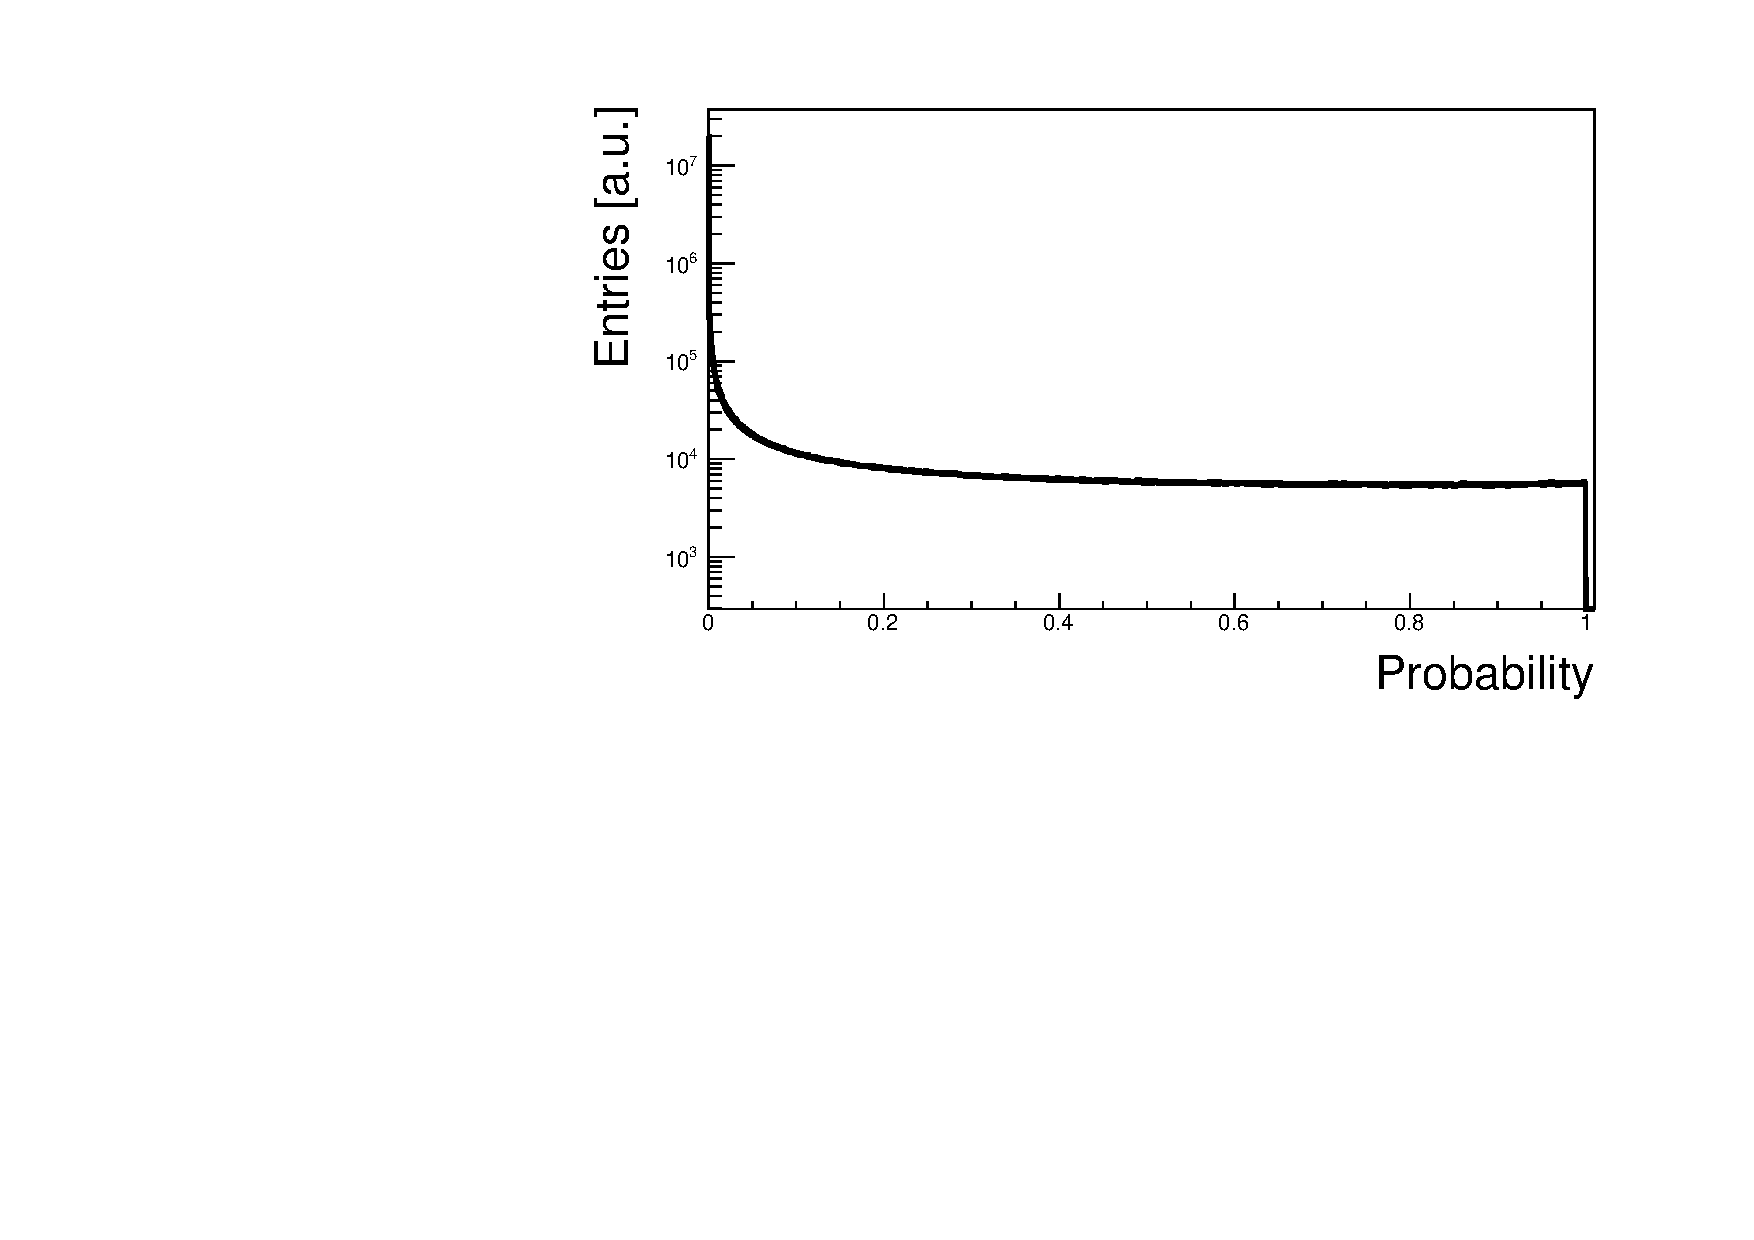
\includegraphics[width=0.47\textwidth]{figures/eta_KFit_Prob.pdf}
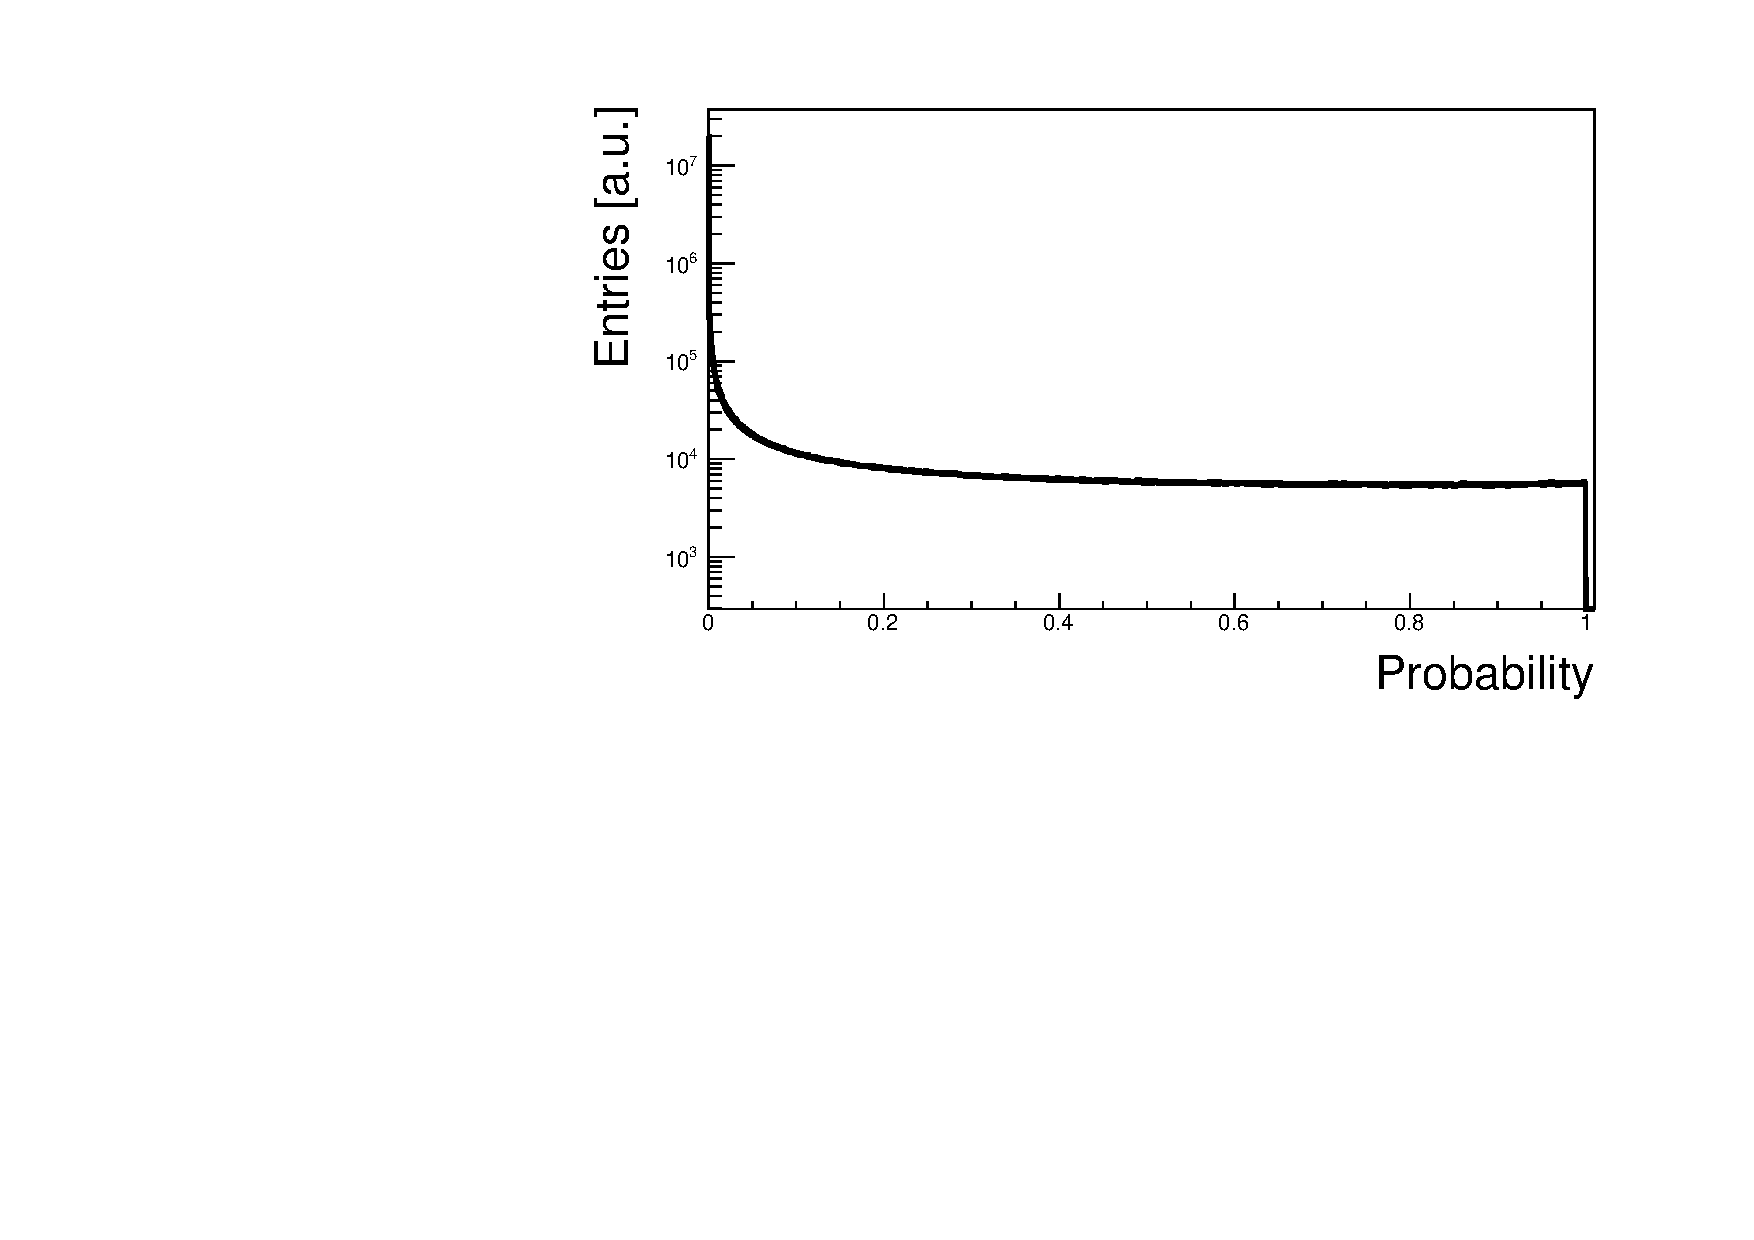
\includegraphics[width=0.47\textwidth]{figures/eta_KFit_Prob.pdf}
\caption{\label{fig:kinfitperform}
(Left) ...
 (Color online)}
\end{center}
\end{figure}

\subsection{Particle identification \label{sec:perfpid}}

Particle identification in GlueX uses information from both energy loss in different detector systems and time-of-flight measurements.  This information can be used for identification in several ways.  The simplest method is to apply selections directly on the relevant PID variables.  To include detector resolution information, one can create a $\chi^2$ variable comparing a measured value to the expected value for a particular hypothesis, that is
\begin{equation}
    \chi^2(p) = \left(  \frac{ X(\mathrm{measured}) - X(\mathrm{expected})_p}{\sigma_X} \right)
\end{equation}
where $X$ is the given PID variable, $p$ is the particle hypothesis, and $\sigma_X$ is the resolution of this variable.  Finally, multiple PID variables can be combined into one probability, or other figure-of-merit (FOM).   Standard, loose selections on time-of-flight and energy loss are sufficient for initialize physics analyses, while the performance of more complicated selections is being actively studied.

At sufficiently large $\theta$, the energy loss ($dE/dx$) for charged particles in the central drift chamber can be used.   Fig.~\ref{fig:performcdcdedx} illustrates these distributions for positively charged particles, showing a clear separation of pions and protons in the momentum range $\lesssim 1$~GeV. % along with the standard selection used to separate pions and protons.

\begin{figure}[tbp]
\begin{center}
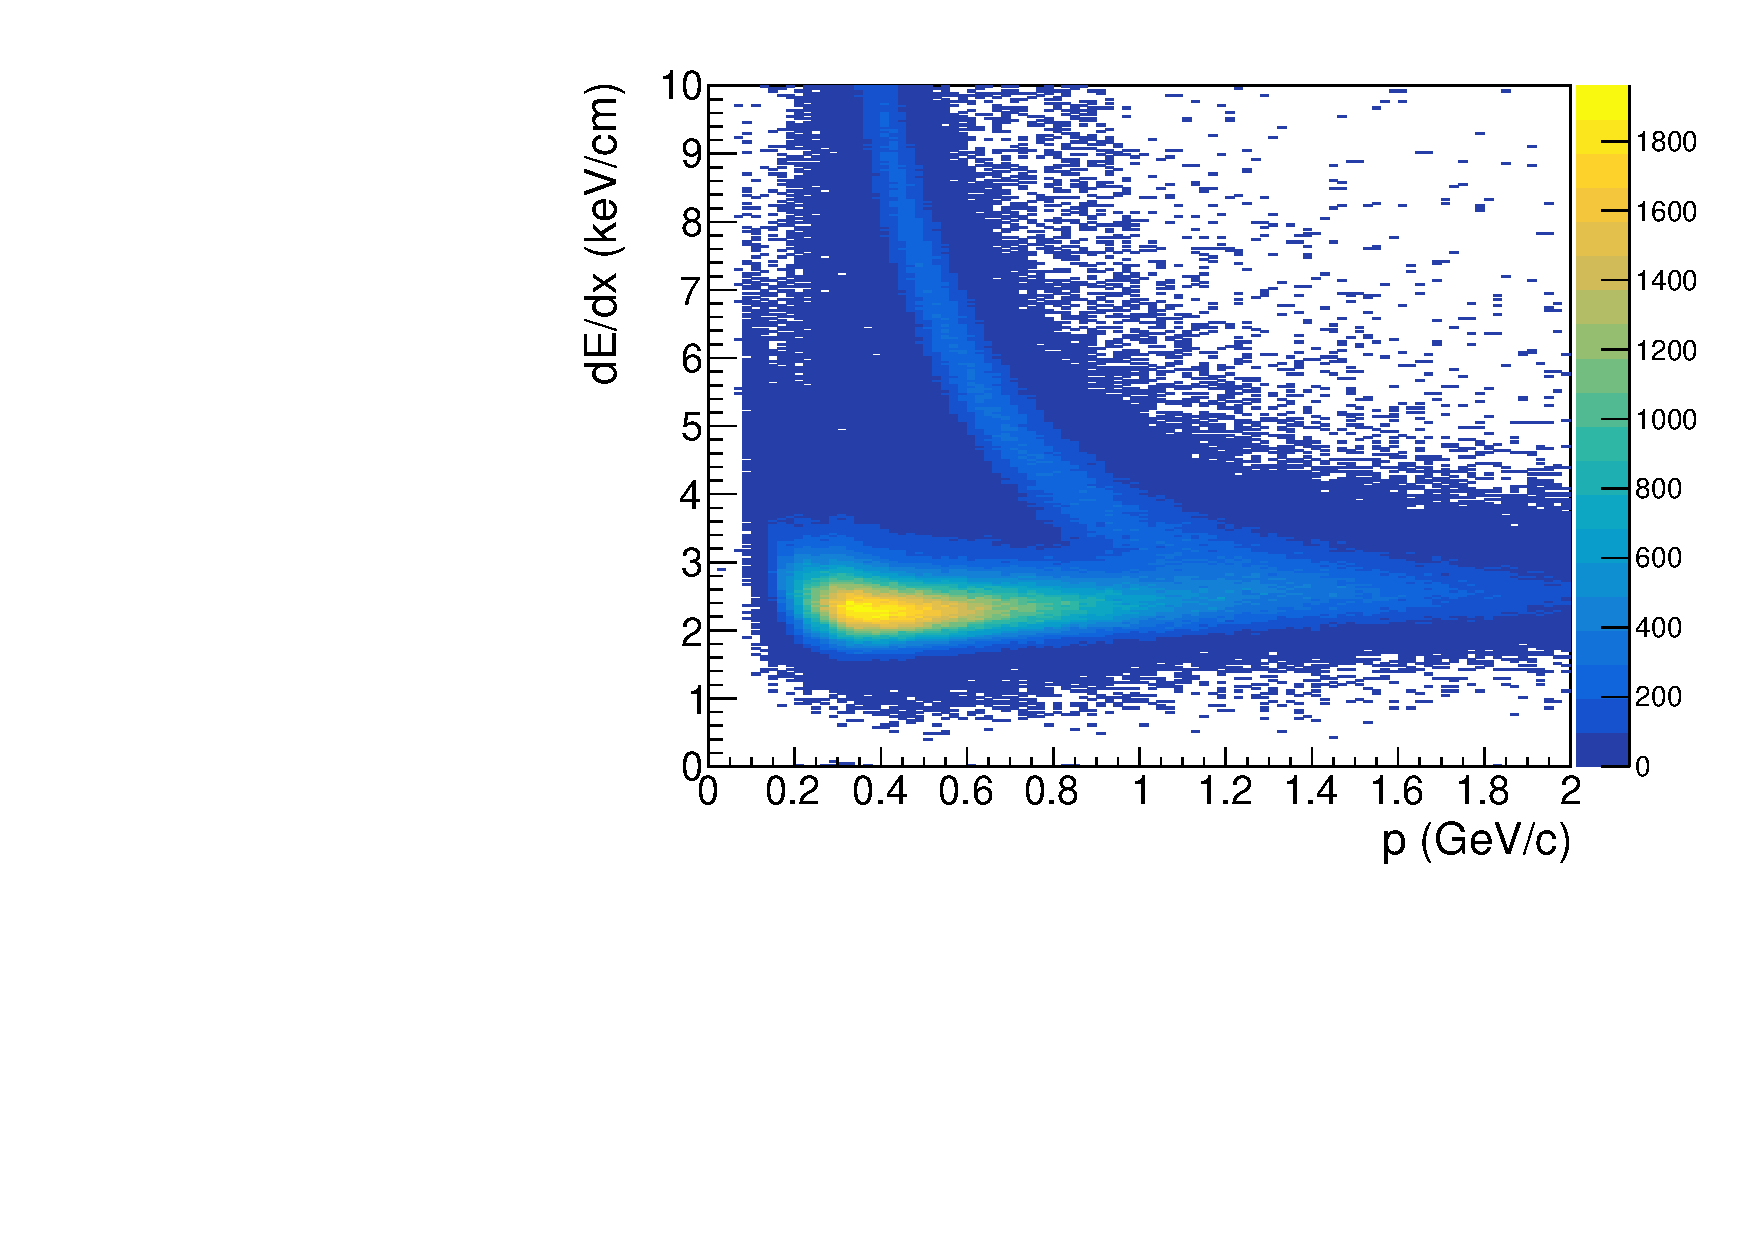
\includegraphics[width=0.6\textwidth]{figures/cdc_pos_dedx.pdf}
\caption{\label{fig:performcdcdedx}
CDC energy loss ($dE/dx$) for positively charged particles that have at least 8 hits in the detector as a function of measured particle momentum.  The band corresponding to protons curves upwards, showing a larger energy loss than pions and other lighter particles at low momentum.  The two bands show a clear separation for momenta  $\lesssim 1$~GeV.
}
\end{center}
\end{figure}

The primary means of particle identification is through time of flight measurements, and information from several sources are combined to make the most accurate determination.  The RF reference signal from the accelerator is used to time when each photon bunch enters the target.  The reconstructed final state particles are used to determine which photon bunch most likely generated the detected reaction, with the primary determination being the signals from the Start Counter associated with the charged particle tracks.  This photon bunch determination has a resolution of around 15~ps?. Each charged particle is associated with additional timing information based on the hit in the highest resolution detector that it is associated with, for example the BCAL or TOF.  The time of flight to this measured hit ($t_\mathrm{meas.}$) from the time of the photon bunch that generated the event ($t_\mathrm{RF})$ can be used to distinguish between differently massed particles.  Two common variables that are used are the velocity ($\beta$) determined using the measured time-of-flight and the momentum of the particle, and $\Delta t_\mathrm{RF}$, the difference between the measured and RF times described above after they both have been extrapolated back to the center of the target, assuming some particle hypothesis.
Some illustrations are given in the associated figures.

Electrons are currently primarily identified using the ratio of their energy loss in the electromagnetic calorimeters ($E$) to the momentum reconstructed in the drift chambers ($p$).  This $E/p$ ratio should be approximately 1 for electrons and generally less for hadrons.  This is illustrated in some sample of particles for Fig.~X.  Other variables, such as the shape of the showers generated by the charged particles in the calorimeter, promise to provide additional information to separate electron and hadron showers.

Particle identification and mis-identification rates are summarized in Fig.~X.

%\subsection{Systematic uncertainties \label{sec:systematics}}
